\documentclass[12pt,a4paper]{report}
\usepackage[utf8]{inputenc}
\usepackage[T1]{fontenc}
\usepackage{graphicx}
\usepackage{hyperref}
\usepackage{geometry}
\usepackage{booktabs}
\usepackage{listings}
\usepackage{xcolor}
\usepackage{amsmath}
\usepackage{float}
\usepackage{titlesec}

\geometry{
    top=2.5cm,
    bottom=2.5cm,
    left=3cm,
    right=2.5cm
}

\lstset{
    basicstyle=\ttfamily\small,
    keywordstyle=\color{blue},
    stringstyle=\color{red},
    commentstyle=\color{green!60!black},
    frame=single,
    breaklines=true,
    captionpos=b,
    numbers=left,
    numberstyle=\tiny\color{gray}
}

\title{
    \vspace{2cm}
    \textbf{\Huge Information Retrieval System}\\
    \vspace{0.5cm}
    \textbf{\Large dengan Word2Vec Query Expansion}
}
\author{
    \textbf{Kelompok 7}\\
    
\includegraphics[width=0.5\textwidth]{images/itb.jpg}
    \vspace{0.5cm}
    Orvin Andika Ikhsan Abhista (13523017)\\
    Fajar Kurniawan (13523027)\\
    Salman Hanif (13523056)\\
    Aryo Wisanggeni (13523100)\\
    Sabilul Huda (13523072)
}
\date{\today}

\begin{document}

\maketitle
\thispagestyle{empty}

\begin{figure}[H]
    \centering
    
\includegraphics[width=0.8\textwidth]{images/itb.jpg}
    \caption{Foto Anggota Kelompok}
\end{figure}

\newpage
\tableofcontents
\newpage

% ============================================================================
\chapter{Pendahuluan}
% ============================================================================

\section{Latar Belakang}
Information Retrieval (IR) adalah proses pengambilan dokumen yang relevan dari koleksi besar berdasarkan query pengguna. Sistem IR konvensional menggunakan pencocokan kata kunci yang sering kali gagal menangkap makna semantik dari query.

Word2Vec adalah model embedding kata yang merepresentasikan kata dalam ruang vektor berdimensi tinggi, di mana kata-kata dengan makna serupa berada berdekatan. Dengan memanfaatkan Word2Vec untuk query expansion, sistem dapat menambahkan kata-kata semantik yang relevan ke query awal, sehingga meningkatkan recall tanpa mengorbankan precision secara signifikan.

Proyek ini mengimplementasikan sistem IR dengan fitur query expansion berbasis Word2Vec menggunakan dataset CISI (Collection of Scientific Information) yang berisi 1460 dokumen dan 112 query uji.

\section{Tujuan}
\begin{enumerate}
    \item Mengimplementasikan sistem IR berbasis TF-IDF cosine similarity
    \item Mengintegrasikan Word2Vec untuk semantic query expansion
    \item Mengevaluasi performa sistem menggunakan Mean Average Precision (MAP)
    \item Membandingkan hasil retrieval antara query original dan query expanded
\end{enumerate}

\section{Ruang Lingkup}
\begin{itemize}
    \item Dataset: CISI collection (1460 dokumen, 112 query, 76 query dengan qrels)
    \item Preprocessing: Lowercasing, tokenization, stopword removal, Porter stemming
    \item Ranking: TF-IDF dengan cosine similarity
    \item Query Expansion: Word2Vec Google News 300 dimensions
    \item Evaluasi: Mean Average Precision (MAP)
\end{itemize}

% ============================================================================
\chapter{Deskripsi Aplikasi}
% ============================================================================

\section{Gambaran Umum}
Sistem ini adalah aplikasi Information Retrieval yang memungkinkan pengguna untuk:
\begin{itemize}
    \item Mencari dokumen dari koleksi CISI menggunakan query teks
    \item Melihat hasil retrieval dengan dan tanpa query expansion
    \item Mengeksplorasi term-term semantik yang ditambahkan oleh Word2Vec
    \item Melihat evaluasi MAP untuk perbandingan performa
\end{itemize}

\section{Fitur Utama}
\begin{enumerate}
    \item \textbf{Document Parsing} - Parser untuk format dokumen CISI (.I, .T, .A, .W, .B tags)
    \item \textbf{Text Preprocessing} - Normalisasi, tokenisasi, stopword removal, stemming
    \item \textbf{Inverted Index} - Pembangunan indeks terbalik untuk pencarian efisien
    \item \textbf{TF-IDF Retrieval} - Ranking dokumen menggunakan TF-IDF cosine similarity
    \item \textbf{Word2Vec Query Expansion} - Penambahan term semantik menggunakan model Word2Vec
    \item \textbf{MAP Evaluation} - Evaluasi performa menggunakan Mean Average Precision
    \item \textbf{REST API} - Endpoint API menggunakan FastAPI
    \item \textbf{Web Interface} - Frontend interaktif (React/Vite)
\end{enumerate}

\section{Arsitektur Sistem}
\begin{figure}[H]
    \centering
    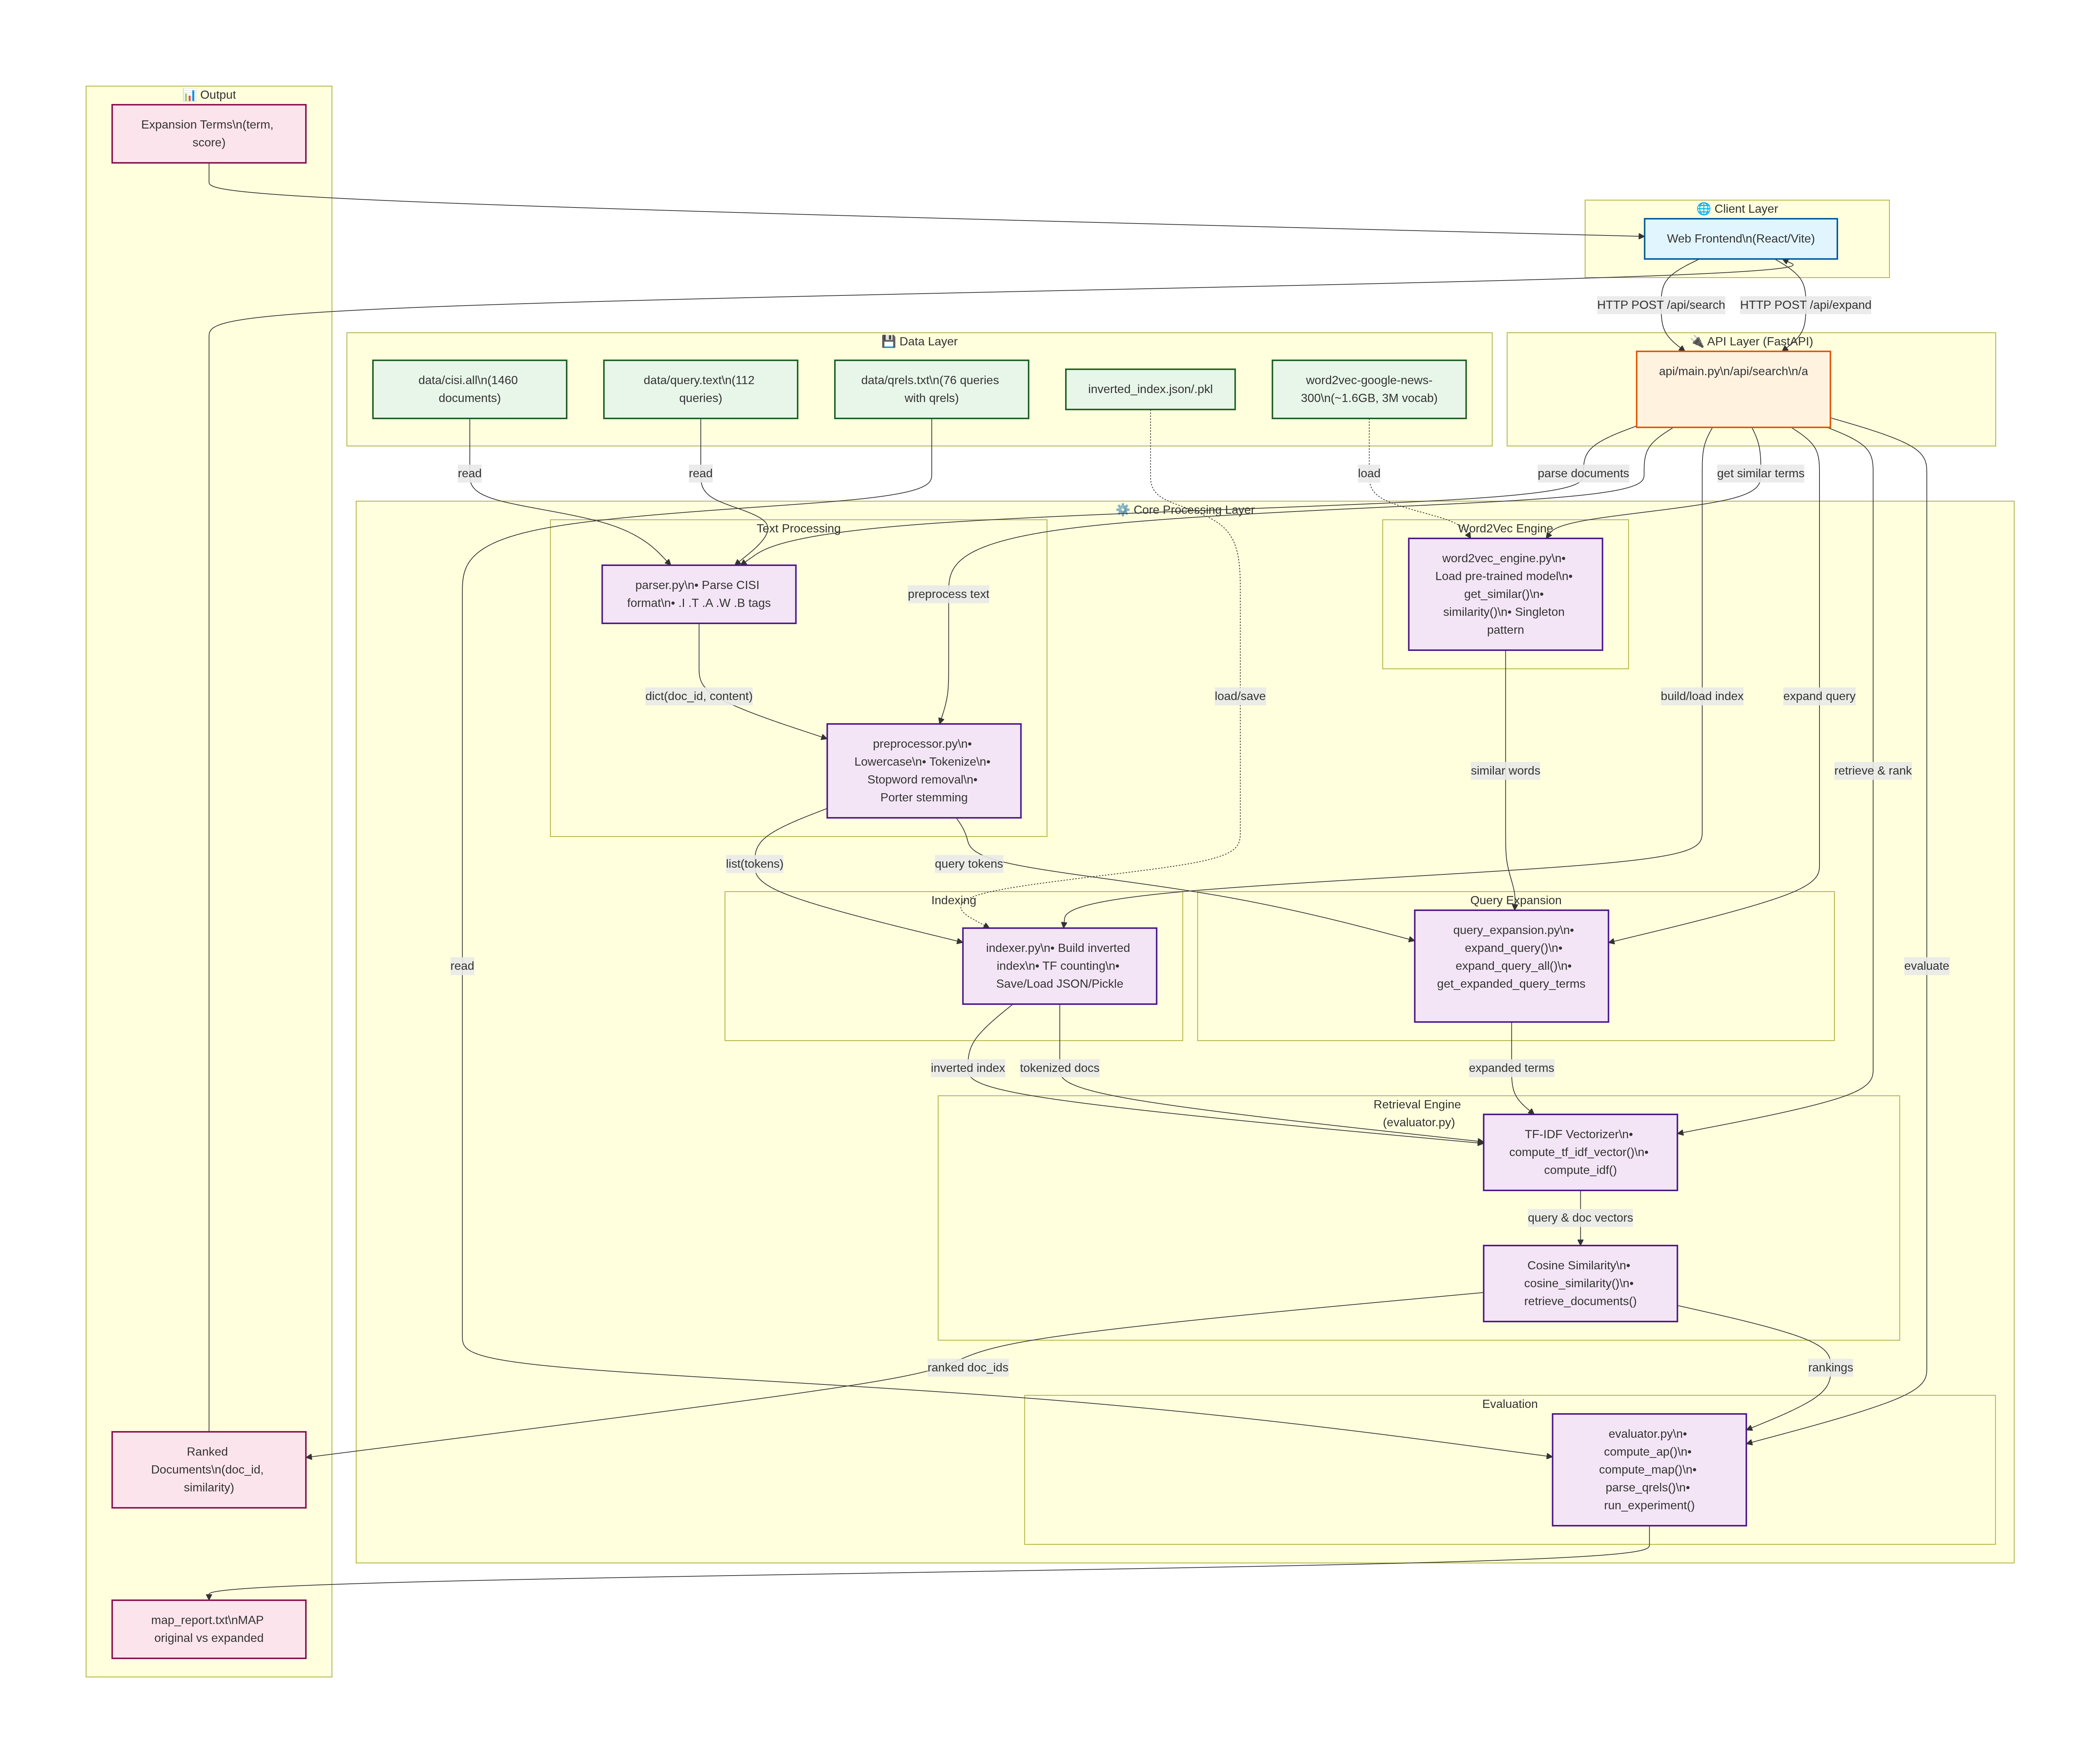
\includegraphics[width=0.8\textwidth]{images/architecture.png}
    \caption{Diagram Arsitektur Sistem}
\end{figure}

Alur data sistem:
\begin{enumerate}
    \item User memasukkan query melalui web interface
    \item Query dipreprocess (tokenize, stem, remove stopwords)
    \item Word2Vec engine mencari term semantik serupa
    \item Query expanded digunakan untuk retrieval TF-IDF
    \item Hasil diurutkan berdasarkan cosine similarity
    \item Hasil ditampilkan dengan perbandingan original vs expanded
\end{enumerate}

% ============================================================================
\chapter{Deskripsi Program}
% ============================================================================

\section{Struktur Proyek}
\begin{lstlisting}[language=bash, caption=Struktur Direktori]
InformationRetrievalSystem-Word2Vec/
+-- src/
|   +-- __init__.py
|   +-- preprocessor.py      # Text preprocessing
|   +-- parser.py            # CISI document parser
|   +-- indexer.py           # Inverted index builder
|   +-- word2vec_engine.py   # Word2Vec model wrapper
|   +-- query_expansion.py   # Query expansion logic
|   \-- evaluator.py         # MAP evaluation
+-- api/
|   \-- main.py              # FastAPI REST API
+-- frontend/                # React web interface
+-- data/
|   +-- cisi.all             # Document collection
|   +-- query.text           # Test queries
|   \-- qrels.txt            # Relevance judgments
+-- main.py                  # Entry point
\-- pyproject.toml           # Dependencies
\end{lstlisting}

\section{Modul Program}

\subsection{preprocessor.py}
Modul ini menangani preprocessing teks dengan fungsi-fungsi:
\begin{itemize}
    \item \texttt{preprocess(text, stemming, remove\_stopword)} - Fungsi utama preprocessing
    \item \texttt{\_normalize\_text(text)} - Lowercase dan hapus karakter non-alfanumerik
    \item \texttt{\_tokenize(text)} - Split teks menjadi token
    \item \texttt{\_remove\_stopwords(tokens)} - Hapus stopwords English (NLTK)
    \item \texttt{\_stem\_tokens(tokens)} - Porter Stemmer
\end{itemize}

\subsection{parser.py}
Parser untuk format dokumen CISI:
\begin{itemize}
    \item \texttt{parse\_docs(file\_path)} - Parse dokumen dari file
    \item \texttt{parse\_text(raw)} - Parse dokumen dari string
    \item Tags yang didukung: \texttt{.I} (ID), \texttt{.T} (Title), \texttt{.A} (Author), \texttt{.W} (Abstract), \texttt{.B} (Bibliography)
    \item Output: \texttt{dict[doc\_id, content]}
\end{itemize}

\subsection{indexer.py}
Pembangunan inverted index:
\begin{itemize}
    \item \texttt{build\_index(docs)} - Build inverted index dari koleksi dokumen
    \item \texttt{save\_index(index, file\_path)} - Simpan index ke JSON/Pickle
    \item \texttt{load\_index(file\_path)} - Load index dari file
    \item \texttt{get\_document\_terms(index, doc\_id)} - Get terms untuk dokumen tertentu
\end{itemize}

\subsection{word2vec\_engine.py}
Wrapper untuk model Word2Vec:
\begin{itemize}
    \item \texttt{init\_engine()} - Inisialisasi singleton engine
    \item \texttt{get\_engine()} - Get engine instance
    \item \texttt{Word2VecEngine.get\_similar(term, top\_n)} - Get semantically similar terms
    \item \texttt{Word2VecEngine.similarity(term1, term2)} - Cosine similarity dua kata
    \item \texttt{Word2VecEngine.train()} - Train model dari koleksi dokumen
    \item Filter: lowercase only, no underscores, min length 3, no substring matches
\end{itemize}

\subsection{query\_expansion.py}
Logika query expansion:
\begin{itemize}
    \item \texttt{expand\_query(query\_terms, top\_n)} - Expand dengan batas term
    \item \texttt{expand\_query\_all(query\_terms)} - Expand tanpa batas
    \item \texttt{get\_expanded\_query\_terms()} - Get combined original + expanded terms
    \item \texttt{format\_expansion\_detail()} - Format output untuk logging
\end{itemize}

\subsection{evaluator.py}
Evaluasi performa sistem:
\begin{itemize}
    \item \texttt{parse\_qrels(file\_path)} - Parse relevance judgments (auto-detect format)
    \item \texttt{compute\_ap(rankings, relevant\_docs)} - Average Precision per query
    \item \texttt{compute\_map(rankings, qrels)} - Mean Average Precision
    \item \texttt{run\_experiment()} - Run full experiment (original vs expanded)
    \item \texttt{write\_report(results)} - Write evaluation report
\end{itemize}

\section{Alur Program}
\begin{enumerate}
    \item \textbf{Inisialisasi}: Load Word2Vec model via \texttt{init\_engine()}
    \item \textbf{Parsing}: Parse dokumen CISI menjadi \texttt{dict[doc\_id, content]}
    \item \textbf{Preprocessing}: Tokenize, stem, remove stopwords
    \item \textbf{Indexing}: Build inverted index dengan term frequencies
    \item \textbf{IDF Computation}: Hitung IDF untuk setiap term
    \item \textbf{Query Processing}:
    \begin{enumerate}
        \item Preprocess query
        \item Expand query dengan Word2Vec (opsional)
        \item Compute TF-IDF vector untuk query
    \end{enumerate}
    \item \textbf{Retrieval}: Compute cosine similarity dengan semua dokumen
    \item \textbf{Ranking}: Urutkan dokumen berdasarkan similarity score
    \item \textbf{Evaluation}: Hitung MAP menggunakan qrels
\end{enumerate}

% ============================================================================
\chapter{Library dan Dependencies}
% ============================================================================

\section{Python Packages}
\begin{table}[H]
    \centering
    \begin{tabular}{@{}lll@{}}
        \toprule
        \textbf{Package} & \textbf{Versi} & \textbf{Kegunaan} \\
        \midrule
        fastapi & $\geq$0.136.3 & REST API framework \\
        uvicorn & $\geq$0.48.0 & ASGI server \\
        gensim & $\geq$4.4.0 & Word2Vec model implementation \\
        nltk & $\geq$3.9.4 & Tokenization, stopwords, Porter stemmer \\
        pysastrawi & $\geq$1.2.1 & Indonesian stemmer (opsional) \\
        pytest & $\geq$9.0.3 & Testing framework \\
        python-multipart & $\geq$0.0.30 & Form data parsing \\
        \bottomrule
    \end{tabular}
    \caption{Dependencies Python}
\end{table}

\section{Word2Vec Model}
Model yang digunakan: \texttt{word2vec-google-news-300}
\begin{itemize}
    \item Dimensi vektor: 300
    \item Training corpus: Google News (~100 miliar kata)
    \item Vocabulary: ~3 juta kata
    \item Ukuran file: ~1.6 GB
    \item Format: KeyedVectors (binary)
\end{itemize}

\section{Frontend}
% PLACEHOLDER_3: Detail frontend framework
\textbf{[PLACEHOLDER\_3: Detail framework frontend (React/Vite, versi, dependencies)]}

% ============================================================================
\chapter{Hasil Eksperimen}
% ============================================================================

\section{Setup Eksperimen}
\begin{itemize}
    \item \textbf{Dataset}: CISI Collection
    \item \textbf{Jumlah Dokumen}: 1460
    \item \textbf{Jumlah Query}: 112 (76 dengan qrels)
    \item \textbf{Preprocessing}: Stemming = True, Stopword Removal = True
    \item \textbf{Ranking}: TF-IDF Cosine Similarity
    \item \textbf{Retrieval}: Top-100 documents per query
    \item \textbf{Query Expansion}: Top-5 similar terms per query term
\end{itemize}

\section{Metrik Evaluasi}
\subsection{Average Precision (AP)}
Average Precision mengukur kualitas ranking untuk satu query:
\begin{equation}
    AP = \frac{1}{|R|} \sum_{k=1}^{n} P(k) \times rel(k)
\end{equation}
dimana:
\begin{itemize}
    \item $|R|$ = jumlah dokumen relevan
    \item $P(k)$ = precision pada posisi ke-$k$
    \item $rel(k)$ = 1 jika dokumen ke-$k$ relevan, 0 jika tidak
\end{itemize}

\subsection{Mean Average Precision (MAP)}
Mean Average Precision adalah rata-rata AP dari semua query:
\begin{equation}
    MAP = \frac{1}{|Q|} \sum_{q=1}^{|Q|} AP(q)
\end{equation}
dimana $|Q|$ = jumlah query.

\section{Hasil Overall}
\begin{table}[H]
    \centering
    \begin{tabular}{@{}lcc@{}}
        \toprule
        \textbf{Metrik} & \textbf{Original} & \textbf{Expanded} \\
        \midrule
        MAP & 0.1791 & 0.1791 \\
        \bottomrule
    \end{tabular}
    \caption{Hasil MAP Overall}
\end{table}

\textbf{Catatan:} Hasil di atas dijalankan tanpa query expansion (Word2Vec model belum di-load). Untuk hasil dengan query expansion, jalankan eksperimen dengan \texttt{use\_expansion=True} setelah menginisialisasi Word2Vec engine.

\section{Hasil Per-Query}
\begin{table}[H]
    \centering
    \small
    \begin{tabular}{@{}lcc@{}}
        \toprule
        \textbf{Query} & \textbf{AP Original} & \textbf{Relevant Docs} \\
        \midrule
        1 & 0.2809 & 46 \\
        2 & 0.0094 & 26 \\
        3 & 0.2216 & 44 \\
        4 & 0.0674 & 8 \\
        5 & 0.0162 & 24 \\
        10 & 0.2796 & 26 \\
        11 & 0.0727 & 127 \\
        20 & 0.0319 & 144 \\
        44 & 0.1110 & 155 \\
        50 & 0.3016 & 89 \\
        52 & 0.7053 & 15 \\
        55 & 0.8625 & 18 \\
        62 & 0.5986 & 12 \\
        65 & 0.4708 & 13 \\
        66 & 0.4796 & 35 \\
        97 & 0.5507 & 6 \\
        102 & 0.4578 & 24 \\
        109 & 0.2014 & 71 \\
        111 & 0.5788 & 6 \\
        \bottomrule
    \end{tabular}
    \caption{Sample Hasil AP Per-Query (Top Queries)}
\end{table}

\section{Analisis Perbandingan MAP Original vs Expanded}
% PLACEHOLDER_4: Analisis lengkap setelah menjalankan eksperimen dengan query expansion
\textbf{[PLACEHOLDER\_4: Analisis perbandingan MAP original vs expanded query]}

\textit{Template analisis yang perlu diisi setelah menjalankan eksperimen dengan Word2Vec:}
\begin{enumerate}
    \item Apakah query expansion meningkatkan MAP? Berapa persen perubahannya?
    \item Query mana yang mengalami peningkatan signifikan? Mengapa?
    \item Query mana yang mengalami penurunan? Mengapa?
    \item Apakah ada pola tertentu pada query yang beneficia dari expansion?
    \item Bagaimana trade-off antara recall dan precision?
\end{enumerate}

\section{Screenshot Aplikasi}
\begin{figure}[H]
    \centering
    % PLACEHOLDER_5: Screenshot halaman utama aplikasi
    \fbox{\parbox{0.8\textwidth}{\centering\vspace{3cm}\textbf{[PLACEHOLDER\_5: Screenshot Halaman Utama]}\vspace{3cm}}}
    \caption{Tampilan Halaman Utama Aplikasi}
\end{figure}

\begin{figure}[H]
    \centering
    % PLACEHOLDER_6: Screenshot hasil pencarian
    \fbox{\parbox{0.8\textwidth}{\centering\vspace{3cm}\textbf{[PLACEHOLDER\_6: Screenshot Hasil Pencarian]}\vspace{3cm}}}
    \caption{Tampilan Hasil Pencarian}
\end{figure}

\begin{figure}[H]
    \centering
    % PLACEHOLDER_7: Screenshot query expansion
    \fbox{\parbox{0.8\textwidth}{\centering\vspace{3cm}\textbf{[PLACEHOLDER\_7: Screenshot Query Expansion]}\vspace{3cm}}}
    \caption{Tampilan Query Expansion}
\end{figure}

% ============================================================================
\chapter{Pembagian Tugas}
% ============================================================================

\section{Anggota Kelompok}
\begin{table}[H]
    \centering
    \begin{tabular}{@{}lllc@{}}
        \toprule
        \textbf{NIM} & \textbf{Nama} & \textbf{Role} & \textbf{File Utama} \\
        \midrule
        13523017 & Orvin Andika Ikhsan Abhista & Programmer 1 & \texttt{preprocessor.py}, \texttt{parser.py} \\
        13523027 & Fajar Kurniawan & Programmer 2 & \texttt{indexer.py} \\
        13523056 & Salman Hanif & Programmer 3 & \texttt{word2vec\_engine.py} \\
        13523100 & Aryo Wisanggeni & Programmer 4 & \texttt{query\_expansion.py} \\
        13523072 & Sabilul Huda & Programmer 5 & \texttt{evaluator.py}, Laporan \\
        \bottomrule
    \end{tabular}
    \caption{Pembagian Tugas Anggota Kelompok}
\end{table}

\section{Detail Tugas}

\subsection{Programmer 1 - Orvin Andika Ikhsan Abhista (13523017)}
\textbf{Tanggung Jawab:} Preprocessing dan Parsing
\begin{itemize}
    \item Implementasi text normalization (lowercase, remove punctuation)
    \item Implementasi tokenization
    \item Integrasi NLTK stopwords removal
    \item Integrasi Porter Stemmer
    \item Parser format dokumen CISI (.I, .T, .A, .W, .B tags)
    \item Normalisasi document ID ke format DOC\#\#\#
\end{itemize}

\subsection{Programmer 2 - Fajar Kurniawan (13523027)}
\textbf{Tanggung Jawab:} Inverted Index
\begin{itemize}
    \item Build inverted index dari koleksi dokumen
    \item Term frequency counting
    \item Document frequency tracking
    \item Save/load index (JSON dan Pickle format)
    \item Document terms retrieval
\end{itemize}

\subsection{Programmer 3 - Salman Hanif (13523056)}
\textbf{Tanggung Jawab:} Word2Vec Engine
\begin{itemize}
    \item Wrapper Word2Vec model (gensim)
    \item Load pre-trained model dari gensim downloader
    \item Train model dari koleksi dokumen
    \item Implementasi \texttt{get\_similar()} dengan filtering
    \item Implementasi \texttt{similarity()} untuk dua kata
    \item Singleton pattern untuk engine instance
\end{itemize}

\subsection{Programmer 4 - Aryo Wisanggeni (13523100)}
\textbf{Tanggung Jawab:} Query Expansion
\begin{itemize}
    \item Implementasi \texttt{expand\_query()} dengan Word2Vec
    \item Implementasi \texttt{expand\_query\_all()} untuk unlimited expansion
    \item Implementasi \texttt{get\_expanded\_query\_terms()} helper
    \item Format expansion detail untuk output
    \item Handling OOV (out-of-vocabulary) terms
\end{itemize}

\subsection{Programmer 5 - Sabilul Huda (13523072)}
\textbf{Tanggung Jawab:} Evaluasi dan Laporan
\begin{itemize}
    \item Implementasi \texttt{compute\_ap()} untuk Average Precision per query
    \item Implementasi \texttt{compute\_map()} untuk MAP overall
    \item Parser qrels (auto-detect format binary/graded)
    \item Experiment runner (original vs expanded)
    \item Report generation
    \item Koordinasi penulisan laporan
    \item Programmer's Reference
\end{itemize}

% ============================================================================
\chapter{Kesimpulan}
% ============================================================================

\section{Kesimpulan}
% PLACEHOLDER_8: Kesimpulan akhir setelah eksperimen lengkap
\textbf{[PLACEHOLDER\_8: Kesimpulan akhir setelah menjalankan eksperimen dengan query expansion]}

\textit{Template yang perlu diisi:}
\begin{itemize}
    \item Apakah sistem IR berhasil diimplementasikan?
    \item Bagaimana performa sistem (MAP score)?
    \item Apakah query expansion memberikan peningkatan?
    \item Apa kelebihan dan kekurangan sistem ini?
\end{itemize}

\section{Saran Pengembangan}
\begin{enumerate}
    \item Implementasi relevance feedback (Rocchio algorithm)
    \item Penambahan ranking algorithm BM25
    \item Support untuk dataset lain (Cranfield, Medline)
    \item Optimasi performa dengan index caching
    \item Docker containerization untuk deployment
    \item Unit tests coverage $>$ 80\%
    \item UI/UX improvement pada frontend
\end{enumerate}

% ============================================================================
\chapter{Lampiran}
% ============================================================================

\section{Cara Menjalankan Program}

\subsection{Instalasi}
\begin{lstlisting}[language=bash]
# Install dependencies
uv sync

# Download NLTK data
python -c "import nltk; nltk.download('stopwords'); nltk.download('punkt')"
\end{lstlisting}

\subsection{Menjalankan API Server}
\begin{lstlisting}[language=bash]
uv run uvicorn api.main:app --reload --host 0.0.0.0 --port 8000
\end{lstlisting}

\subsection{Menjalankan Evaluasi}
\begin{lstlisting}[language=bash]
uv run python -m src.evaluator
\end{lstlisting}

\subsection{Menjalankan dengan Query Expansion}
\begin{lstlisting}[language=python]
from src.word2vec_engine import init_engine
from src.evaluator import run_experiment

init_engine()  # Load Word2Vec model
results = run_experiment(use_expansion=True)
\end{lstlisting}

\section{API Endpoints}
\begin{itemize}
    \item \texttt{GET /} - Health check
    \item \texttt{POST /api/search} - Search dengan query expansion
    \item \texttt{POST /api/expand} - Preview expansion terms
    \item \texttt{GET /api/index/\{doc\_id\}} - Get inverted index
    \item \texttt{GET /api/map} - Get MAP evaluation report
\end{itemize}

\section{Referensi}
\begin{enumerate}
    \item Mikolov, T., et al. (2013). "Efficient Estimation of Word Representations in Vector Space." ICLR.
    \item Robertson, S.E., et al. (1994). "Okapi at TREC-3." TREC.
    \item Manning, C.D., Raghavan, P., \& Schütze, H. (2008). "Introduction to Information Retrieval." Cambridge University Press.
    \item CISI Dataset: \url{https://ir.dcs.gla.ac.uk/resources/test_collections/cisi}
    \item Gensim Documentation: \url{https://radimrehurek.com/gensim/}
    \item NLTK Documentation: \url{https://www.nltk.org/}
    \item FastAPI Documentation: \url{https://fastapi.tiangolo.com/}
\end{enumerate}

\section{Foto Anggota}
% PLACEHOLDER_9: Foto individual anggota kelompok
\begin{figure}[H]
    \centering
    \fbox{\parbox{0.3\textwidth}{\centering\vspace{2cm}\textbf{[PLACEHOLDER\_9a: Foto Orvin Andika]}\vspace{2cm}}}
    \caption{Orvin Andika Ikhsan Abhista (13523017)}
\end{figure}

\begin{figure}[H]
    \centering
    \fbox{\parbox{0.3\textwidth}{\centering\vspace{2cm}\textbf{[PLACEHOLDER\_9b: Foto Fajar Kurniawan]}\vspace{2cm}}}
    \caption{Fajar Kurniawan (13523027)}
\end{figure}

\begin{figure}[H]
    \centering
    \fbox{\parbox{0.3\textwidth}{\centering\vspace{2cm}\textbf{[PLACEHOLDER\_9c: Foto Salman Hanif]}\vspace{2cm}}}
    \caption{Salman Hanif (13523056)}
\end{figure}

\begin{figure}[H]
    \centering
    \fbox{\parbox{0.3\textwidth}{\centering\vspace{2cm}\textbf{[PLACEHOLDER\_9d: Foto Aryo Wisanggeni]}\vspace{2cm}}}
    \caption{Aryo Wisanggeni (13523100)}
\end{figure}

\begin{figure}[H]
    \centering
    \fbox{\parbox{0.3\textwidth}{\centering\vspace{2cm}\textbf{[PLACEHOLDER\_9e: Foto Sabilul Huda]}\vspace{2cm}}}
    \caption{Sabilul Huda (13523072)}
\end{figure}

\end{document}
